\documentclass{article}
\usepackage{graphicx}
\usepackage{float}

\title{Human Computer Interaction \\ Coursework 2}
\author{Shaw Eastwood, s.eastwood@rgu.ac.uk}

\begin{document}
	\maketitle

	\section{Initial Scenario Based Designs}

	\section{table0}
\hspace{-1cm}
	\centering
	\begin{tabular}{p{4cm}p{10cm}}
		\hline
		Title & tourism app \\
		\hline
		Date & 16th April 2019 \\
		\hline
		Scene & 1 of 4 \\
		\hline
		Description & This is the landing page \\
		\hline
		Links From Scenes & N/A \\
		\hline
		Links To Scenes & Scene 2 \\
		\hline
		\multicolumn{2}{c}{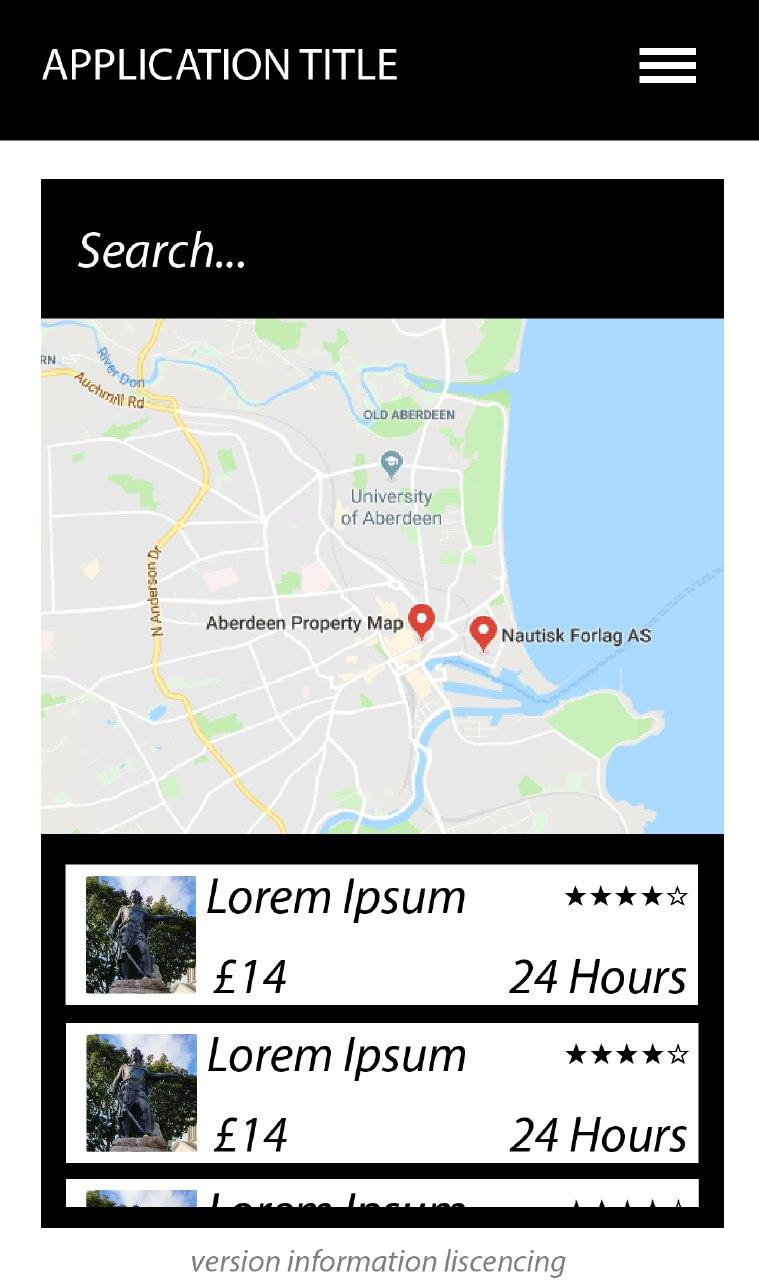
\includegraphics[width=0.5\linewidth]{images/screen0.jpg}} \\
		\hline
		Background & Standard phone background \\
		\hline
		Colour Scehemes Used & Default to black and white but would import from the system theme so users feel immersed \\
		\hline
		Text Attributes & Again, follows system theme (usually a sans-serif font). \\
		\hline
		Audio Files & N/A \\
		\hline
		Video Files & N/A \\
		\hline
		Stills Files & N/A \\
		\hline
		Animations / Movie Clips & N/A \\
		\hline
		\multicolumn{2}{c}{Interface Components (buttons, widgets)} \\
		\hline
		\multicolumn{2}{p{14cm}}{The interface consists of a number of bold, large buttons for the user to choosefrom linking to the various, primary, function of the app} \\
		\hline
	\end{tabular}

	\hspace{-1cm}
	\begin{tabular}{p{4cm}p{10cm}}
		\hline
		Title & tourism app \\
		\hline
		Date & 16th April 2019 \\
		\hline
		Scene & 2 of 4 \\
		\hline
		Description & The search page of the application \\
		\hline
		Links From Scenes & Scene 1, Scene 3 \\
		\hline
		Links To Scenes & Scene 3 \\
		\hline
		\multicolumn{2}{c}{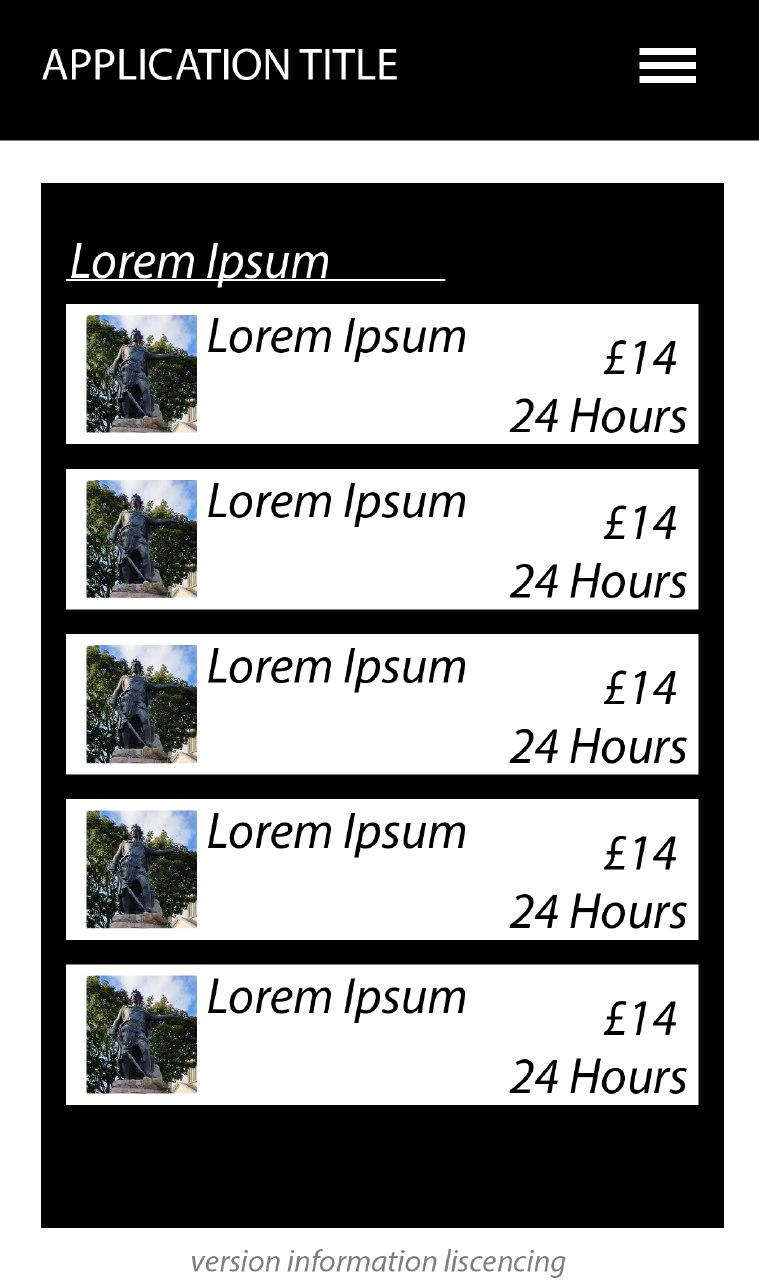
\includegraphics[width=0.5\linewidth]{images/screen1.jpg}} \\
		\hline
		Background & Standard phone background \\
		\hline
		Colour Scehemes Used & Default to black and white but would import from the system theme so users feel immersed \\
		\hline
		Text Attributes & Again, follows system theme (usually a sans-serif font). \\
		\hline
		Audio Files & N/A \\
		\hline
		Video Files & N/A \\
		\hline
		Stills Files & N/A \\
		\hline
		Animations / Movie Clips & N/A \\
		\hline
		\multicolumn{2}{c}{Interface Components (buttons, widgets)} \\
		\hline
		\multicolumn{2}{p{14cm}}{ This page shows a list of "card"-esque locations that match the search term provided by the user on the main page. Above them is the search box that the user can see their current search and make an edit to it.  } \\
		\hline
	\end{tabular}

	\hspace{-1cm}
	\centering
	\begin{tabular}{p{4cm}p{10cm}}
		\hline
		Title & tourism app \\
		\hline
		Date & 16th April 2019 \\
		\hline
		Scene & 3 of 4 \\
		\hline
		Description & The selected page \\
		\hline
		Links From Scenes & Scene 1, Scene 2 \\
		\hline
		Links To Scenes & Scene 1, Scene 2 \\
		\hline
		\multicolumn{2}{c}{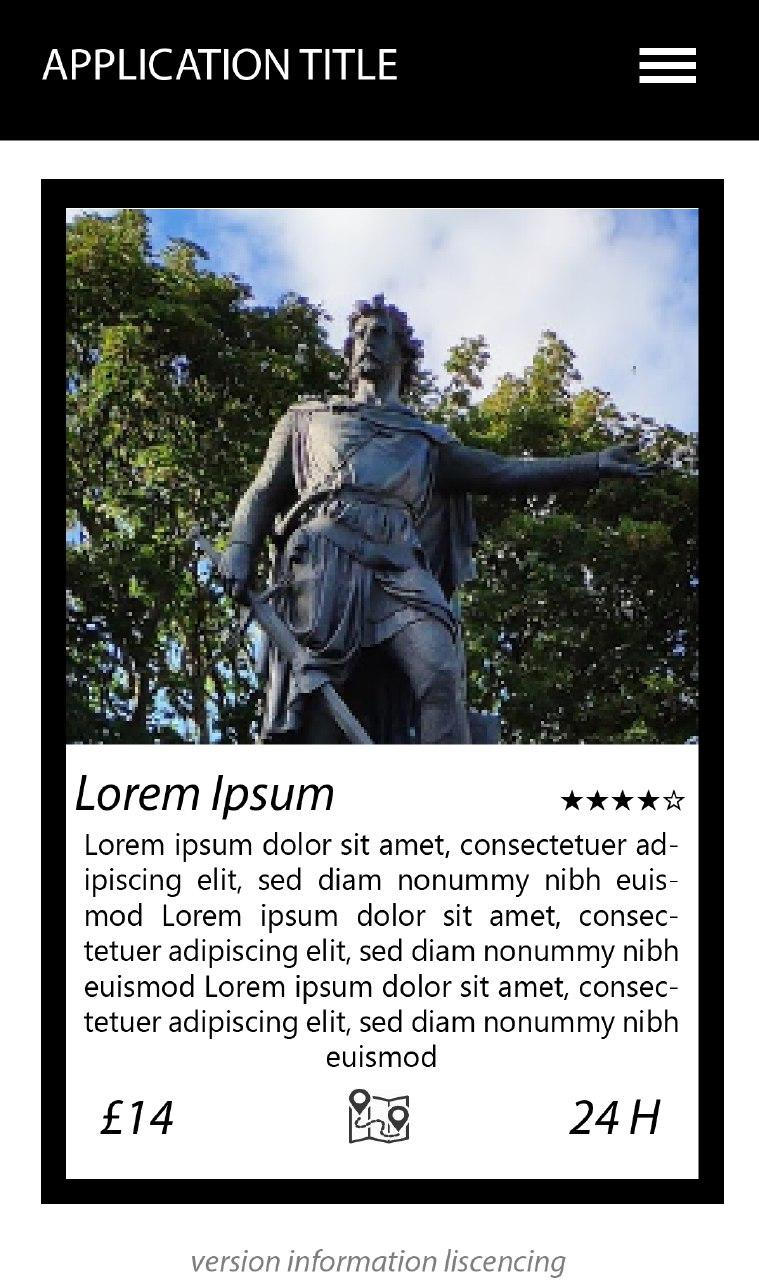
\includegraphics[width=0.5\linewidth]{images/screen2.jpg}} \\
		\hline
		Background & Solid white background on black to highlight the "card design" \\
		\hline
		Colour Scehemes Used & Default to black and white but would import from the system theme so users feel immersed \\
		\hline
		Text Attributes & Again, follows system theme (usually a sans-serif font). \\
		\hline
		Audio Files & N/A \\
		\hline
		Video Files & N/A \\
		\hline
		Stills Files & Header Image for the Location \\
		\hline
		Animations / Movie Clips & N/A \\
		\hline
		\multicolumn{2}{c}{Interface Components (buttons, widgets)} \\
		\hline
		\multicolumn{2}{p{14cm}}{This page contains all of the relevant information pertaining to the attraction. The main content is the image of the location selected by either votes of users or by the maintainers of the attraction. Following this is the Title and the rating on the same line. The rating is powered by user feedback. Next is the description of the attraction of the site which again is chosen by the maintainers. Finally on at the bottom is the price of the venue, a link to get directions to the site and the opening hours.} \\
		\hline
	\end{tabular}


	\section{User Feedback}
	The user feedback recieved described in this section will inform the on the final designs on in the next section.
	A series of questions were sent out and users asked to respond on these based on the designs about, below are the results.
\begin{table}[H]
\hspace{-3cm}
	\begin{tabular}{lllcp{3cm}llc}
	\hline
	name & age & occupation & native & question1 & question2 & question3 & question4 \\
	\hline
	Adam & 21 & Student & Yes & Check for transport availability & Yes & Yes & None \\
	Liam & 22 & Student & Yes & Opening times of venue & Yes & No & Have to sign up \\
	Steve & 45 & Mechanic & No & Access by public transport & No & No & Internet Acess \\
	Anne & 24 & Researcher & No & Public Transport access and opening times & No & Yes & the past locations \\
	Luke & 22 & Software Engineer & Yes & Ability to filter by distance, opening times & Yes & Yes & None \\
	James & 20 & Barista & No & Filter by cost/opening times & Yes & Yes & None \\
	Alice & 23 & Developer & No & Only see highly rated locations & Yes & Yes & None \\
	John & 31 & Carpenter & No & Link to the pages website, pictures of the place, make bookings for tours & No & Yes & Tracking of any kind \\
	Bill & 29 & IT & Yes & If the place has food onsite, if not nearby locations & Yes & Yes & None \\
	\hline
\end{tabular}
\end{table}
	As observed from the results above we can see that the primary concerns are mostly covered by our current design but the addition of a "nearby locations" would help increase the user experience.
	Conversely we can see that the decision to not include a profile function in the early prototyping was useful as some respondents raised concerns with data collection.
	However a number of the core features, such as the rating and the photo adding will require this feature.
\section{CogTool}


\end{document}
